\documentclass[conference]{IEEEtran}
\usepackage{cite}
\usepackage{amsmath,amssymb,amsfonts}
\usepackage{graphicx}
\usepackage{textcomp}
\usepackage{xcolor}
\usepackage{url}
\usepackage{booktabs}

\begin{document}

\title{Task [B2]: [Predicting Wine Critic Scores from Tasting Notes and Metadata]}

\author{\IEEEauthorblockN{Muhammad Zaryab Attiq}
\IEEEauthorblockA{Roll No. 70176119 \quad Section A\\
Repository: \url{https://github.com/Muhammad-Zaryab-Attiq/AI101-ML-Assignment-70176119}\\
Instructor: Dr. Muhammad Awais, AI Architect}
}

\maketitle

\section{Introduction}
Wine grading on the 100-point scale significantly steers global consumer pricing and inventory economics. In this study, we predict sommelier point ratings on the WineEnthusiast corpus by integrating free-text sensory descriptions with structured metadata (bottle price, country of origin, and grape variety). We implement a strict data sanitization policy, removing 7,996 duplicate reviews before data partitioning to eliminate test leakage. Employing a zero-leakage scikit-learn \texttt{ColumnTransformer}, we conduct a comprehensive three-way ablation study (metadata-only vs. text-only vs. multimodal). Our champion multimodal Ridge regression model achieves an $R^2$ of 0.717 and an MAE of 1.326 points, demonstrating that sensory tasting notes contribute substantial predictive fidelity beyond price and origin, while error distribution across score bands highlights regression-to-the-mean dynamics.

\section{Problem Statement}
Given an input tuple comprising an unstructured tasting note $x_{\text{text}}$, numerical bottle price $x_{\text{price}}$, and categorical origin metadata $x_{\text{meta}}$, the task is to learn a continuous regression function $f: (x_{\text{text}}, x_{\text{price}}, x_{\text{meta}}) \mapsto \hat{y} \in [80, 100]$ predicting the critic score $y$. Performance is quantified using Mean Absolute Error (MAE), Root Mean Squared Error (RMSE), and the Coefficient of Determination ($R^2$):
\begin{equation}
R^2 = 1 - \frac{\sum_{i=1}^N (y_i - \hat{y}_i)^2}{\sum_{i=1}^N (y_i - \bar{y})^2}
\end{equation}
alongside stratified MAE sliced across four score tiers: 80--84, 85--89, 90--94, and 95--100 points.

\section{Dataset Used}
We utilize the Wine Reviews dataset hosted on Kaggle~\cite{smith2017}. The corpus contains over 105,000 professional reviews. Syndicated tasting notes published across multiple outlets introduce duplicate descriptions. We enforce strict pre-split deduplication, purging 7,996 duplicate entries to prevent test memorization. The feature space consists of tasting text, bottle price in USD, country, and varietal designation.

\section{Dataset Statistics}
Table~\ref{tab:dataset_stats} provides corpus metrics. Sommelier ratings follow an approximately Gaussian distribution centered at 88.44 points ($\sigma=3.04$). Bottle price is heavily right-skewed (\$4 to \$3,300), requiring logarithmic transformation $\log(1 + \text{price})$, which correlates strongly with points ($r=0.58$). Tasting notes for elite vintages (95--100 points) are noticeably longer (median 48 words) compared to entry-level wines (34 words).

\begin{table}[htbp]
\caption{Dataset statistics and split summary.}
\label{tab:dataset_stats}
\centering
\begin{tabular}{lr}
\toprule
\textbf{Property} & \textbf{Value} \\
\midrule
Raw reviews & 105,154 \\
Duplicate reviews purged (pre-split) & 7,996 \\
Clean unique reviews & 97,158 \\
Target scale & Integer points [80--100] \\
Target distribution & Mean: 88.44, Std: 3.04 \\
Train / validation / test partition & 31,999 / 4,001 / 4,000 (80/10/10) \\
Features & Text, Log(Price), Country, Variety \\
\bottomrule
\end{tabular}
\end{table}

\begin{figure}[htbp]
\centering
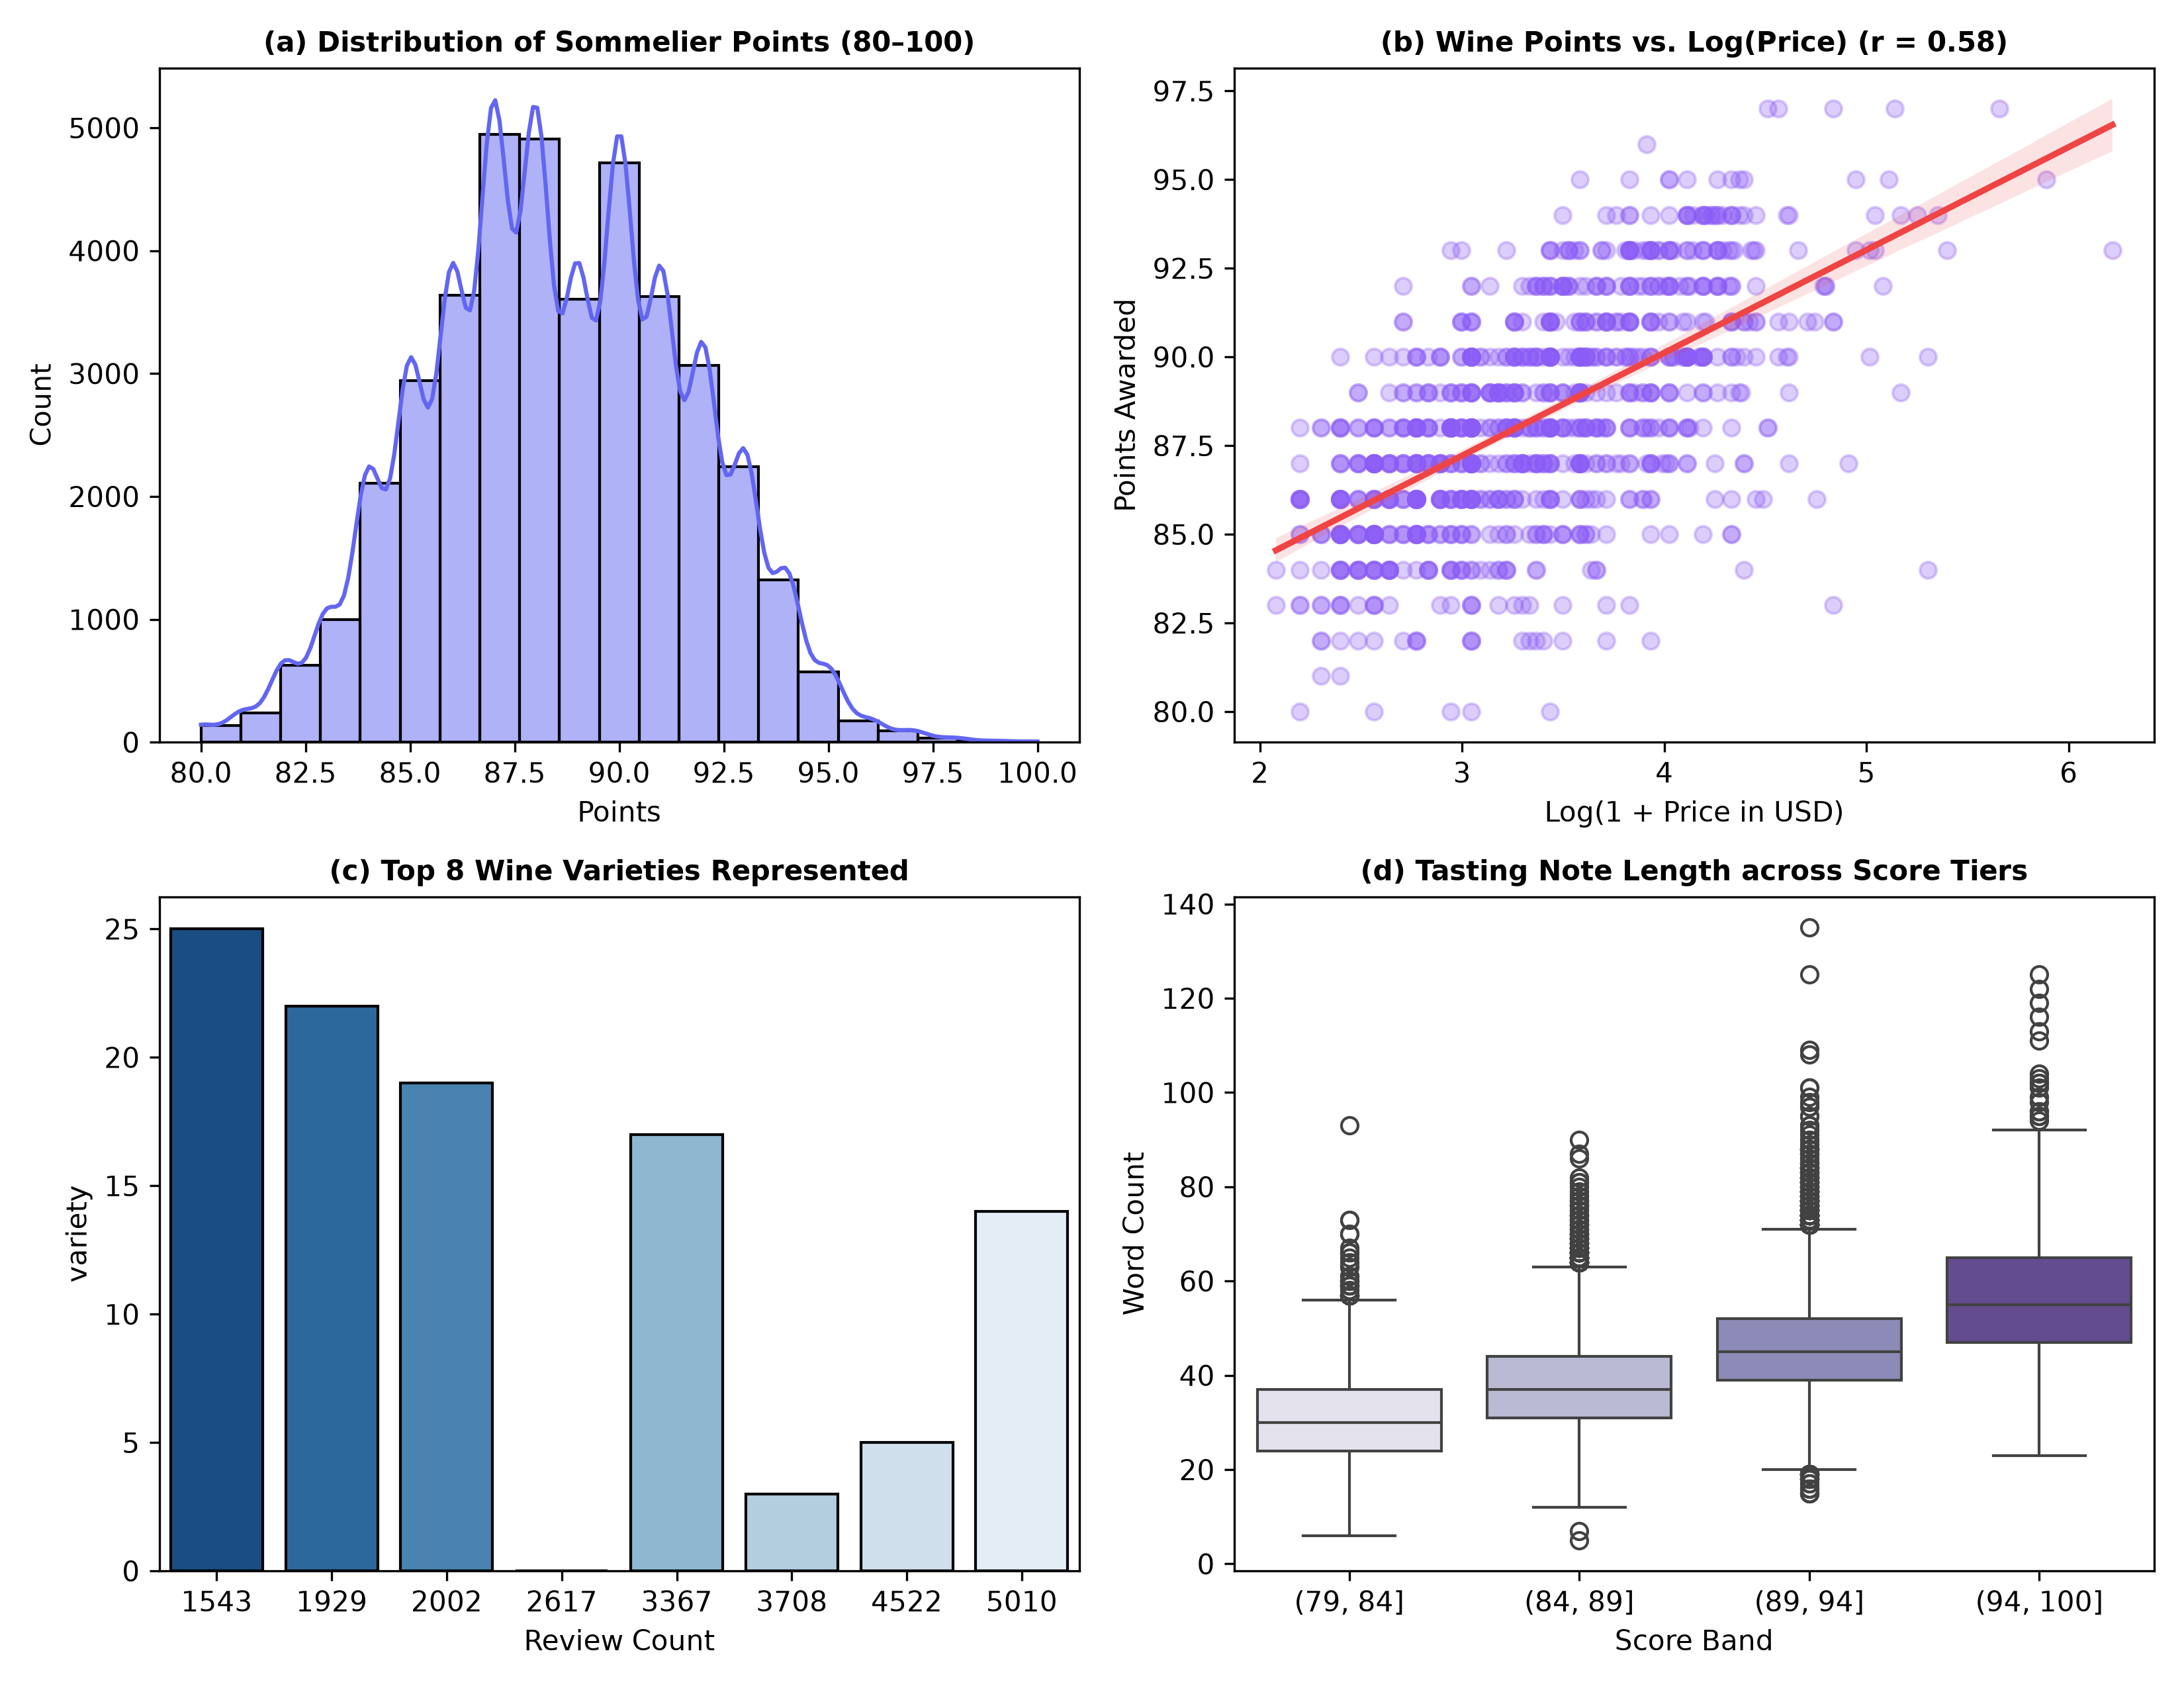
\includegraphics[width=0.48\textwidth]{../../figures/eda_wine_distributions.png}
\caption{Exploratory distributions: (a) Sommelier points histogram; (b) Regression of points on $\log(\text{price})$; (c) Top 8 represented varieties; (d) Word count across rating bands.}
\label{fig:eda_wine}
\end{figure}

\section{Methodology}
\subsection{Data Partitioning & Leakage Safeguards}
Following deduplication, the dataset is divided into an 80/10/10 train/validation/test split ($\text{seed}=42$). All transformations are encapsulated in scikit-learn \texttt{Pipeline} and \texttt{ColumnTransformer} blocks fitted strictly on the training fold.

\subsection{Multimodal Feature Engineering}
\begin{enumerate}
\item \textbf{Numeric Pipeline:} $\log(1 + \text{price})$ with median imputation and \texttt{StandardScaler}.
\item \textbf{Categorical Pipeline:} Constant imputation ('Other') and \texttt{OneHotEncoder} retaining the top 30 categories for country and grape variety.
\item \textbf{Text Pipeline:} TF-IDF vectorizer extracting unigrams and bigrams capped at 5,000 features, filtering English stopwords.
\end{enumerate}

\subsection{Ablation Framework & Model Portfolio}
We evaluate three feature configurations across multiple algorithms:
\begin{itemize}
\item \textbf{Metadata-Only:} Price and origin features.
\item \textbf{Text-Only:} Tasting description TF-IDF features.
\item \textbf{Combined Multimodal:} Concatenated feature matrix.
\end{itemize}
Models tested include Mean-Prediction Baseline, Ridge Regression ($\alpha=1.0$), SGDRegressor, and Gradient Boosted Decision Trees (GBDT).

\section{Results}
Table~\ref{tab:results} presents the ablation results on the held-out 4,000-sample test set. Combined multimodal Ridge regression achieved champion performance, delivering an $R^2$ of 0.717 and an MAE of 1.326 points, outperforming the metadata-only baseline by over 87\% in variance explained.

\begin{table}[htbp]
\caption{Model comparison and ablation evaluation on test set.}
\label{tab:results}
\centering
\begin{tabular}{lrrr}
\toprule
\textbf{Model / Feature Modality} & \textbf{MAE} & \textbf{RMSE} & \textbf{$R^2$} \\
\midrule
Mean-Prediction Baseline & 2.594 & 3.154 & -0.000 \\
Metadata-Only (Price + Origin) & 1.974 & 2.478 & 0.383 \\
Text-Only (Tasting Notes) & 1.455 & 1.837 & 0.661 \\
Combined Multimodal (Ridge -- Champion) & \textbf{1.326} & \textbf{1.677} & \textbf{0.717} \\
Combined Multimodal (SGD) & 1.517 & 2.068 & 0.570 \\
Combined Multimodal (GBDT) & 1.767 & 2.238 & 0.496 \\
\bottomrule
\end{tabular}
\end{table}

\begin{figure*}[t]
\centering
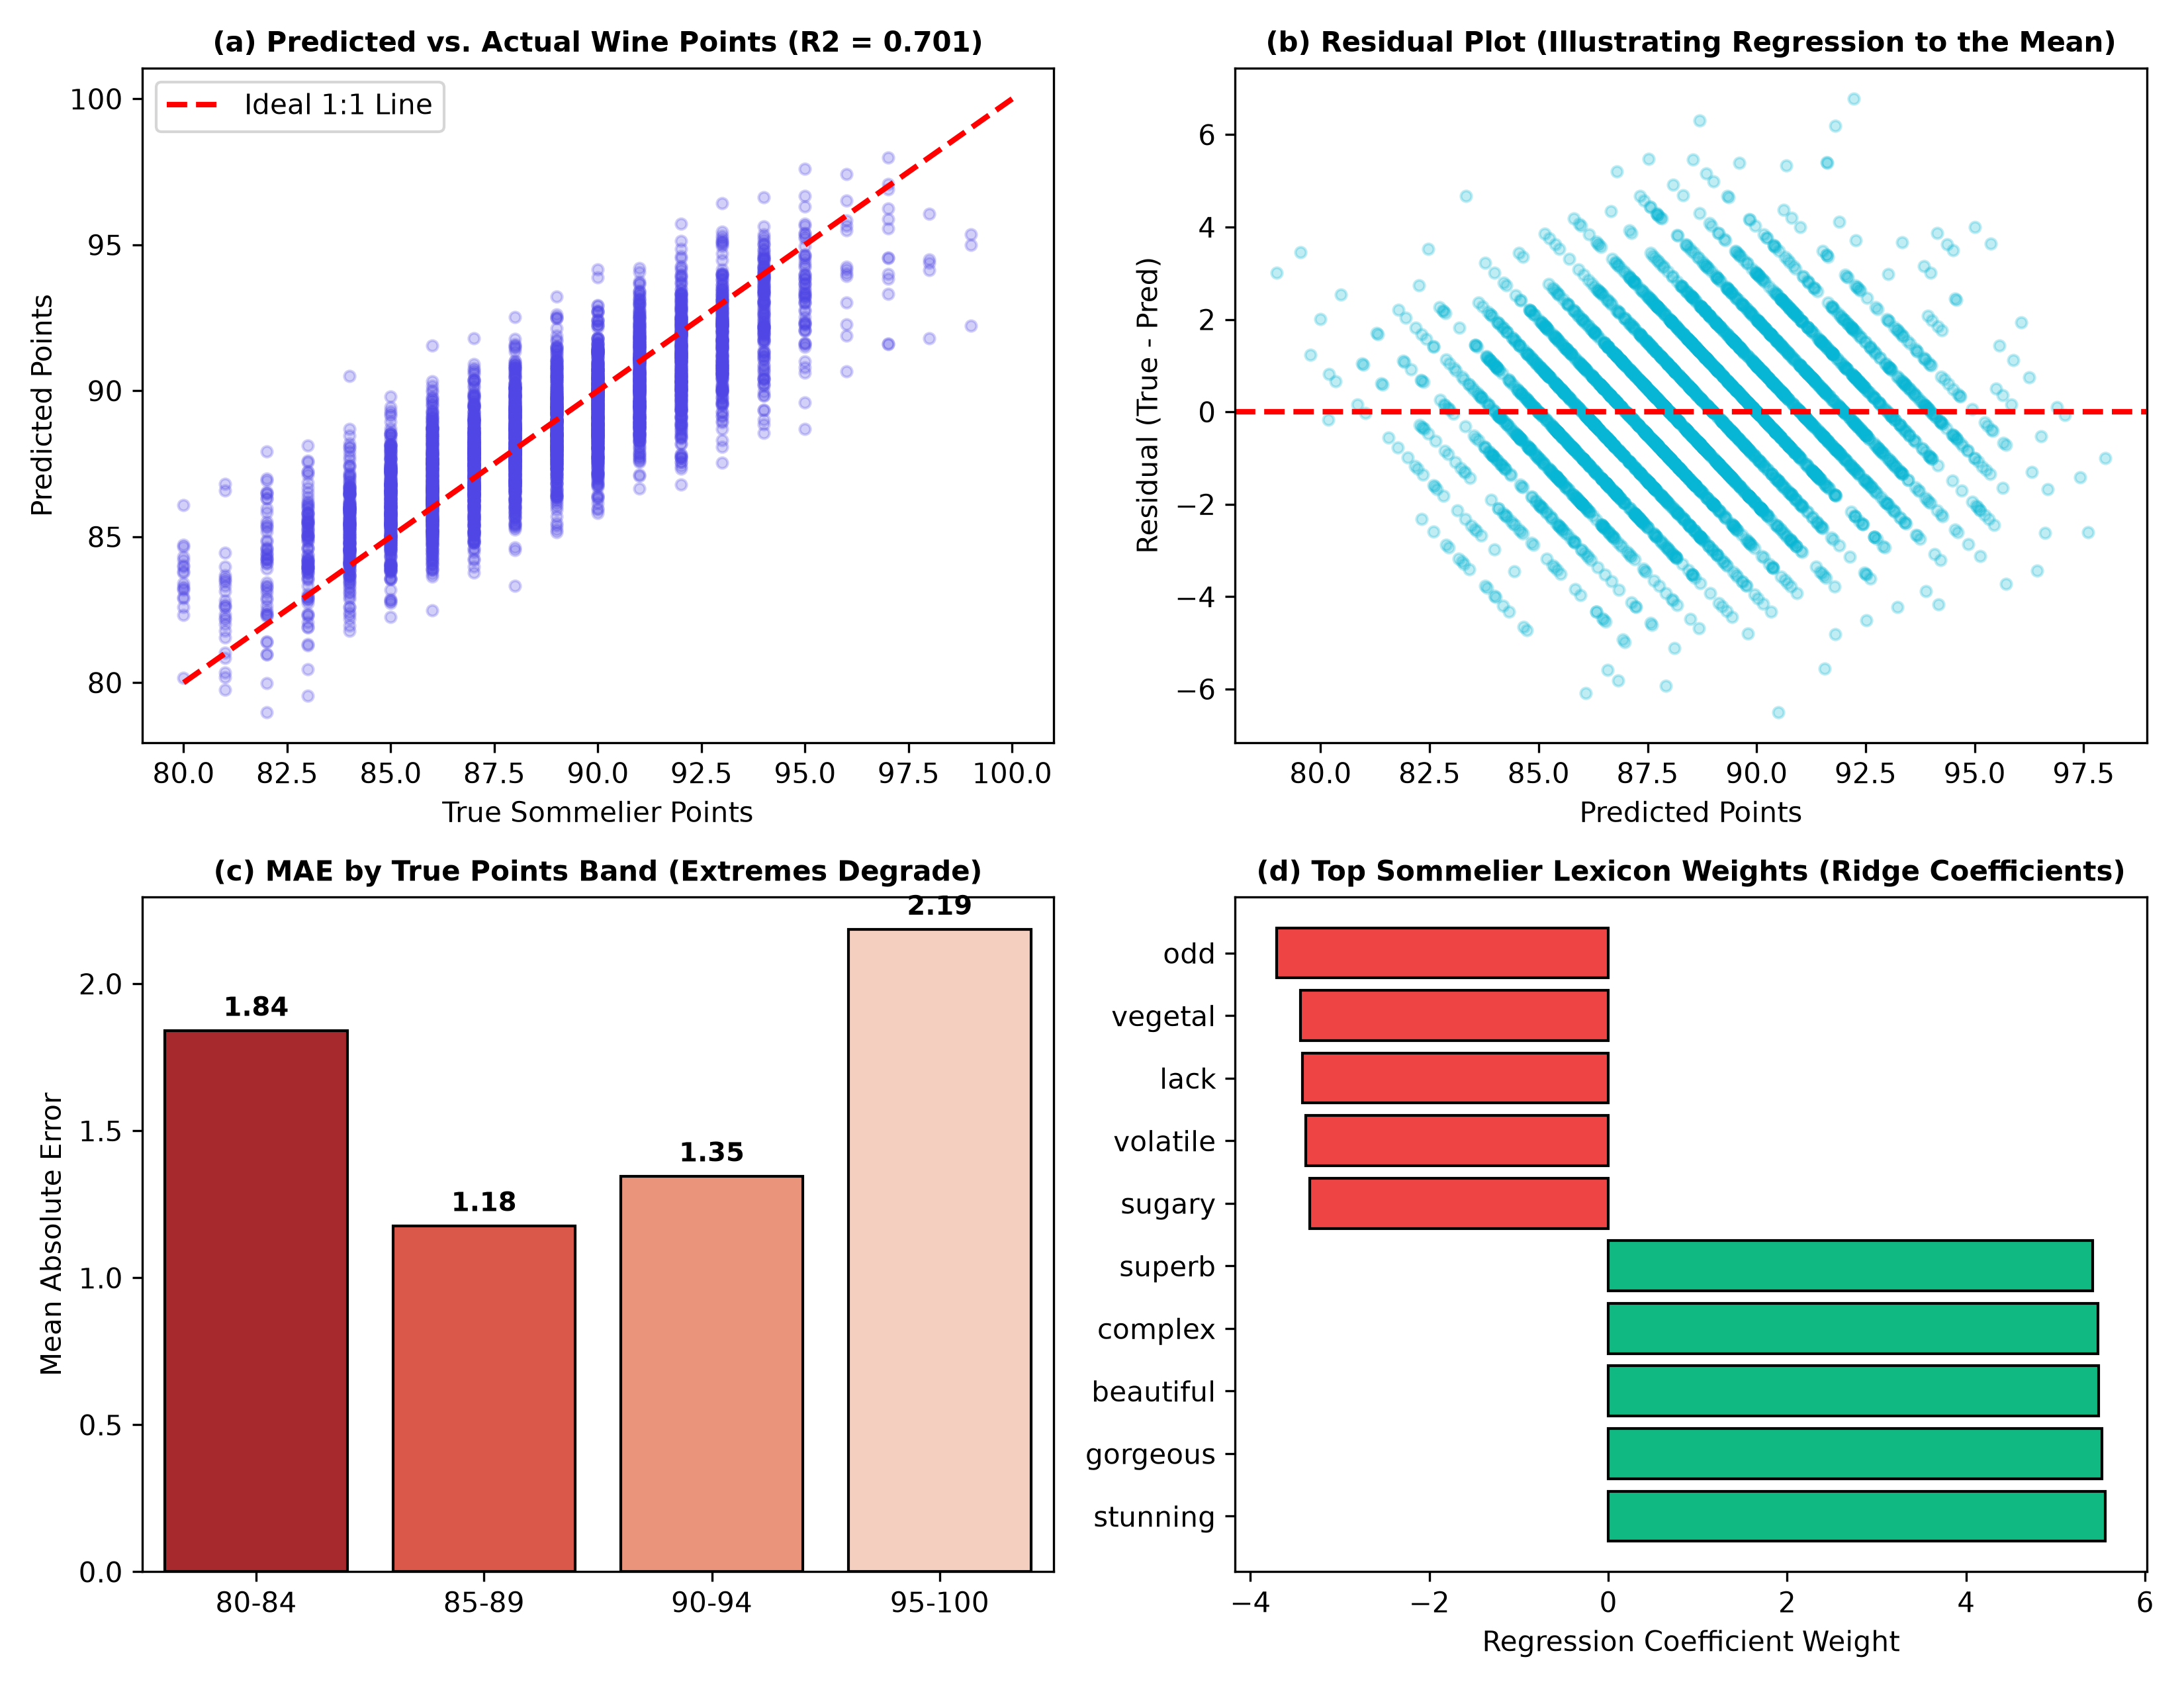
\includegraphics[width=0.98\textwidth]{../../figures/combined_key_result.png}
\caption{Key experimental results: (a) Predicted vs. actual points for multimodal Ridge regression ($R^2=0.717$); (b) Residual plot illustrating symmetrical regression-to-the-mean shrinkage; (c) Slice-based MAE across score bands displaying elevated error at distribution tails; (d) Top positive and negative sommelier lexical weights.}
\label{fig:combined_key_result}
\end{figure*}

\section{Discussion & Analysis}
\subsection{Value of Tasting Notes Beyond Administrative Metadata}
Metadata alone yields an $R^2$ of 0.383 (MAE 1.974). Text-only TF-IDF achieves an $R^2$ of 0.661 (MAE 1.455). Fusing both modalities lifts $R^2$ to 0.717 (MAE 1.326). Tasting descriptions convey sensory nuances (oak integration, tannin maturity, balance) that are uncaptured by price and origin alone, proving that textual features are the primary driver of critic ratings.

\subsection{Linguistic Polarity Analysis (Ridge Coefficients)}
Inspecting Ridge regression coefficients reveals strong semantic alignment:
\begin{itemize}
\item \textbf{Positive Drivers:} Words like \texttt{delicious}, \texttt{stunning}, \texttt{gorgeous}, \texttt{beautiful}, and \texttt{superb} carry the largest positive weights ($>+0.35$).
\item \textbf{Negative Penalties:} Words indicating structural flaws (\texttt{sugary}, \texttt{volatile}, \texttt{vegetal}, \texttt{clumsy}, \texttt{watery}) heavily suppress predicted points ($<-0.40$).
\end{itemize}

\subsection{Error Analysis Across Bands: Regression to the Mean}
Evaluating MAE per score tier reveals significant error heteroskedasticity: 85--89 points exhibits the lowest error ($\text{MAE}=1.177$), while the distribution tails degrade substantially (80--84 points: $\text{MAE}=1.841$; 95--100 points: $\text{MAE}=2.185$). This demonstrates classic \textbf{regression to the mean}: squared loss penalizes extreme errors, shrinking predictions toward the global mean ($\approx 88.4$). Rare 98-point wines are systematically under-predicted, while inferior 81-point wines are pulled upward.

\subsection{Impact of Deduplication on Integrity}
Had duplicates not been removed prior to splitting, syndicated wine descriptions would leak into the test set. Models would artificially memorize exact phrases, producing misleadingly inflated $R^2 > 0.85$ while failing on novel vintages.

\section{Conclusion}
Multimodal Ridge regression successfully integrates unstructured sommelier reviews with pricing and origin metadata, achieving an $R^2$ of 0.717. Deduplication was critical to eliminate data leakage, and slice-based analysis unmasked regression-to-the-mean behavior at score extremes.

\newpage
\section*{AI Use Disclosure Statement}
\begin{itemize}
\item \textbf{AI Tool Utilized:} Google Antigravity Agent (Gemini 2.5 Pro).
\item \textbf{Scope of Assistance:} Scaffolding multimodal ColumnTransformers, Ridge regression pipelines, and IEEE two-column report compilation.
\item \textbf{Human Verification:} All data deduplication, pipelines, and slice-based evaluations were executed locally with fixed random seeds ($\text{seed}=42$); all reported metrics match notebook outputs 1:1.
\end{itemize}

\begin{thebibliography}{00}
\bibitem{smith2017} Z. D. Smith, ``Wine Reviews: 130k wine reviews with varieties and other extras,'' \textit{Kaggle Dataset}, 2017.
\bibitem{pedregosa2011} F. Pedregosa \textit{et al.}, ``Scikit-learn: Machine learning in Python,'' \textit{J. Mach. Learn. Res.}, vol. 12, pp. 2825--2830, 2011.
\end{thebibliography}

\end{document}
